%
% File: chap01.tex
%
\let\textcircled=\pgftextcircled
\chapter{Theory}
\label{chap:intro}

\initial{W}hen refueling a reactor, either with a different loading pattern or with changes in some materials in the core area, the operator does not know when criticality might occur. For example, especially at nuclear reactor, testing of highly reactive fuel rods could happen, in which case a full core's reactivity might excess the control rods worth. A predictive way of getting the criticality information is to compute the subcritical multiplication factor, loading the fuel rods a few at a time, and updating the prediction at each step.

The procedure is issued from handouts from the USGS-Reactor Lab course at the Colorado School of Mines~\cite{reactor01}.

%=======
\section{Source neutrons}
\label{sec:source}

Source neutrons can be produced by different means. They could appear from natural decay of fissile material, in the fuel, from gamma-sources (a ($\gamma - n$) reaction) or from a discrete neutron source placed in the core. In the case of the latter, which is installed at the GSTR facility, it can mask the core criticality by emitting neutrons, and absorbing neutrons depending on the neutron flux.

In one generation, the number of neutrons produced by the discrete source is given by:

\begin{equation}\label{eq1}
N = S k_{eff}
\end{equation}
where:
\begin{conditions}
 N   &  Total neutron population \\
 S   &  Number of source neutrons \\   
 k_{eff} &  Effective multiplication factor ($<1$ for a subcritical core)
\end{conditions}

Consequently, after say two generations, the neutron population is given by:

\begin{equation}\label{eq2}
N = S + S * (k_{eff}) + (S k_{eff}) * k_{eff}
\end{equation}

This series can be written for a number n of generations as:

\begin{equation}\label{eq3}
N = S \frac{1}{1-k_{eff}}
\end{equation}

One can also define the subcritical multiplication factor $M$, as:

\begin{equation}\label{eq4}
M = \frac{N}{S} = \frac{1}{1-k_{eff}}
\end{equation}

And its inverse, which is more convenient and easy to use in this case study:

\begin{equation}\label{eq5}
\frac{1}{M} = 1-k_{eff}
\end{equation}

It is important to note that in a subcritical core, the fission reaction cannot sustain itself. It will die down. One might think that it means that all your neutrons will disappear from your core. But the neutron source keeps emitting neutrons into the core, and at each generation, more source-fission neutrons are added to the system~\ref{app:app01}. Eventually, the power level, i.e. the neutron population in the core, stabilize. As can be seen on figure~\ref{fig:neupop}, the number of generations (time-dependent) needed for the stabilization to occur strongly depends on the effective multiplication factor value, doing so quickly for $k_{eff} = 0.5$ but showing an almost linear correlation for $k_{eff} = 0.99$.

\begin{figure}[t!]
	\centering
	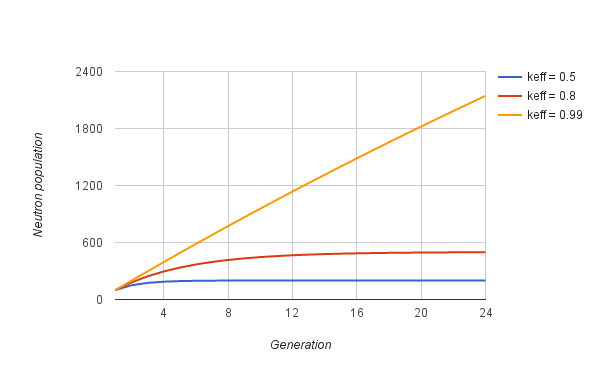
\includegraphics[height=0.4\textheight]{fig01/neupop.png}
	\mycaption[Neutron population with a fixed source at different $k_{eff}$ values]{Neutron population with a fixed source at different $k_{eff}$ values.}
	\label{fig:neupop}
\end{figure}

\section{Neutron count rate}

Sometimes, the reactivity $\rho$ cannot be directly measured, and must be computed from other availbale data. The reactivity is directly correlated to the number of neutrons in the core, and as such to the count rate.


\begin{equation}\label{eq6}
\rho = \frac{k_{eff}-1}{k_{eff}}
\end{equation}


\begin{equation}\label{eq7}
\frac{1}{M} = 1 - k_{eff, c} = \frac{\rho}{\rho - 1} = \frac{CR_i}{CR_c}
\end{equation}
\begin{conditions}
 CR_i   &  Initial count rate \\
 CR_c   &  Current count rate \\
 k_{eff, c}   &  Current effective multiplication factor
\end{conditions}

Plotting $\frac{1}{M}$, i.e. the change in the count rate, as a function of the number of fuel elements in the core, will allow prediction of the number of elements needed to reach criticality.

However, in order for the measurements to be correct, it is necessary to place the source in a position where it won't mask the neutron flux from this addition to the neutron detector. A more detailed point will be made about this in \ref{}.

\section{Procedure}

In preparation of this approach to criticality experiment, fifteen fuel elements were taken from the core. They are identified by serial numbers written on them, but without high quality camera, this is difficult to read. So, careful care is observed when moving the fuel rods in and out of the core, and their positions before and after being moved is traced in the Reactor Operations Logbook and in the Fuel Element History Logbook. When moving several fuel rods in one sitting, the movements must be planned ahead.

Depending on the movements plan to be followed, the neutron source should be moved to a position where it would not interfere with the detector reading, as explicited by figure~\ref{fig:goodbaddet}.

\begin{figure}[t!]
	\centering
	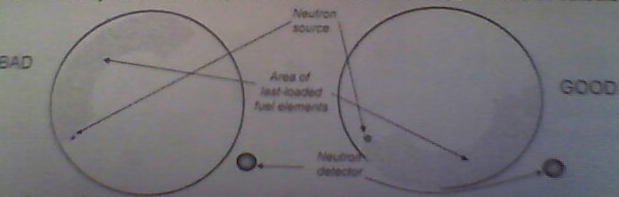
\includegraphics[height=0.2\textheight]{fig01/goodbaddet.png}
	\mycaption[Correct neutron source positioning in the core]{Correct neutron source positioning in the core.}
	\label{fig:goodbaddet}
\end{figure}

To physically move the fuel rods, a manual fuel-handling tool is used. Two persons are usually needed to operate it: one to guide it, and the other to latch or unlatch on its head.

The reactor is in a shutdown state (all control rods down) during any fuel-handling operations.

After a few fuel rods have been inserted back into the core, the control rods are taken to the top, and the relative subcritical multiplication factor can be computed using data from the NM1000. This data is then used to predict the number of fuel elements to be inserted before reaching criticality without control rods. A conservative and step-by-step (not too many fuel rods at once) approach should be adopted, since the first few data points can be misleading.


